%%%%%%%%%%%%%%%%%%%%%%%%%%%%%%%%%%%%%%%%%
% Classicthesis-Styled CV
% LaTeX Template
% Version 1.0 (22/2/13)
%
% This template has been downloaded from:
% http://www.LaTeXTemplates.com
%
% Original author:
% Alessandro Plasmati
%
% License:
% CC BY-NC-SA 3.0 (http://creativecommons.org/licenses/by-nc-sa/3.0/)
%
%%%%%%%%%%%%%%%%%%%%%%%%%%%%%%%%%%%%%%%%%

%----------------------------------------------------------------------------------------
%	PACKAGES AND OTHER DOCUMENT CONFIGURATIONS
%----------------------------------------------------------------------------------------

\documentclass{scrartcl}

\reversemarginpar % Move the margin to the left of the page 

\newcommand{\MarginText}[1]{\marginpar{\raggedleft\itshape\small#1}} % New command defining the margin text style

\usepackage[nochapters]{classicthesis} % Use the classicthesis style for the style of the document
\usepackage[LabelsAligned]{currvita} % Use the currvita style for the layout of the document
\usepackage{graphicx}

\usepackage{wrapfig}
\renewcommand{\cvheadingfont}{\LARGE\color{Maroon}} % Font color of your name at the top

\usepackage{hyperref} % Required for adding links	and customizing them
\hypersetup{colorlinks, breaklinks, urlcolor=Maroon, linkcolor=Maroon} % Set link colors

\newlength{\datebox}\settowidth{\datebox}{2014 - Present} % Set the width of the date box in each block

\newcommand{\NewEntry}[3]{\noindent\parbox{\datebox}{\textit{#1}}\hspace{1.5em} #2 #3 % Define a command for each new block - change spacing and font sizes here: #1 is the left margin, #2 is the italic date field and #3 is the position/employer/location field
\vspace{0.5em}} % Add some white space after each new entry

\newcommand{\Description}[1]{\noindent\footnotesize{#1}\par\normalsize\vspace{1em}} % Define a command for descriptions of each entry - change spacing and font sizes here

\usepackage{color}
\definecolor{lightgray}{gray}{0.9}
\newcommand{\CVSection}[1]{\noindent
  \hspace{-10em}\colorbox{lightgray}{%
  \hspace{10em}\parbox{35em}{\Large \spacedlowsmallcaps{#1}}}
}


%----------------------------------------------------------------------------------------

\begin{document}

\thispagestyle{empty} % Stop the page count at the bottom of the first page

%----------------------------------------------------------------------------------------
%	NAME AND CONTACT INFORMATION SECTION
%----------------------------------------------------------------------------------------

\begin{cv}{\spacedallcaps{Tina Seifpoor}}\vspace{1.5em} % Your name

\date{}
\CVSection{Personal Information}
\begin{wrapfigure}{r}{0.1\textwidth}
\vspace{-0.1in}
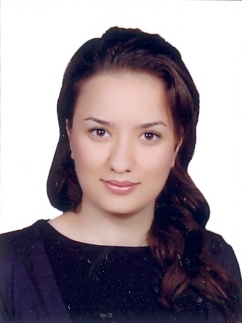
\includegraphics[width=1in]{tina.jpg}
\end{wrapfigure}

\Description{\MarginText{}Iran, 9 September 1984} % Birthplace and date

\Description{\MarginText{E-mail}tina.seifpoor@gmail.com}% Email address

\Description{\MarginText{Address}Bordenbergweg 12, 64367, M\"uhltal} % Personal 

\Description{\MarginText{Cell Phone}+49 (176) 204 23 036} % Phone number(s)

\vspace{1em} % Extra white space between the personal information section and goal

%------------------------------------------------

\vspace{.7cm}

%----------------------------------------------------------------------------------------
%	COMPUTER SKILLS
%----------------------------------------------------------------------------------------

\CVSection{Skills}\vspace{1em}

\Description{\MarginText{General}Signal processing, Network security, Optics, Documentation and design}
\vspace{1em}
\Description{\MarginText{Software}Microsoft Office, Matlab, NS, Deterlab, Adobe Illustrator, Adobe Photoshop}
 
%------------------------------------------------
\vspace{.7cm}
%----------------------------------------------------------------------------------------
%	WORK EXPERIENCE
%----------------------------------------------------------------------------------------

\CVSection{Work Experience}

%------------------------------------------------

\NewEntry{2014--2015}{Marketing Manager, \textsc{CryptTech}}

\Description{\MarginText{CryptTech Co.}Technical and customer documentation and presentation of network security products (Network monitoring, SIEM, log management and hotspot). \\Reference: Alper \textsc{Yilmaz}\ \ $\cdotp$\ \ \href{alperyilmaz@crypttech.com}{alperyilmaz@crypttech.com}}

%------------------------------------------------

\NewEntry{2010--2013}{Researcher, \textsc{ADAX Project}}

\Description{\MarginText{Bogazici University}Member of research team in ADAX -- attack detection and counter-measures simulation -- developing solutions to detect complex attacks against information systems. \\ Reference: Prof. Emin \textsc{Anarim}\ \ $\cdotp$\ \ \href{anarim@boun.edu.tr}{anarim@boun.edu.tr}}

%------------------------------------------------

\NewEntry{2008--2010}{Sales Manager, \textsc{F.R.S. Co.}}

\Description{\MarginText{F.R.C. Co.}Customer Relations Manager, Operational Management, Export/Import Organizer  \\ Reference: Mr. Rahim \textsc{Alijani}\ \ $\cdotp$\ \ \href{info@rockstone.biz}{info@rockstone.biz}}

%------------------------------------------------

\vspace{.7cm}

%----------------------------------------------------------------------------------------
%	EDUCATION
%----------------------------------------------------------------------------------------

\CVSection{Education}\vspace{1em}

\NewEntry{2014-\small frozen}{Bogazici University, Istanbul}

\Description{\MarginText{Doctor of Philosophy}School: Electrical \& Electronics Engineering Dept.\newline 
Thesis: \textit{Application of Self-Interference Lloyd's Fiber Interferometer in pressure and bending sensors}\newline
Description: Interference fringes of reflections from Lloyd can be used to observe pressure or bending of an optic fiber and the application of it will be investigated experimentally.\newline
Advisor: Assoc. Prof.~Heba \textsc{Yuksel}
\\Subjects:
\begin{itemize}
  \item Free Space Optical Communications
  \item Fiber Optics
  \item Light Fidelity (Li-Fi)- Visible light communication 
\end{itemize}
}

\NewEntry{2010-2013}{Bogazici University, Istanbul}

\Description{\MarginText{Master of Science}GPA: 3.25/4\ \ $\cdotp$\ \ School: Electrical \& Electronics Engineering Dept.\newline 
Thesis: \textit{Active filtering against DDoS attacks}\newline
Description: This thesis explored the idea of providing security for the networks against known network DDoS(Distributed denial of service) attack by detecting and filtering the malicious packets by means of analyzing statistical features and Bloom filter. Other subject are Stochastic signal processing, Image processing and analysis and wireless network and mobile systems. \newline
Advisor: Prof.~Emin \textsc{Anarim}
\\Subjects:
\begin{itemize}
  \item Statistical Signal Analysis
  \item Cryptology \& Network Securty
  \item Detection and Estimation Theory
  \item Information Systems Security Principles
\end{itemize}
}

%------------------------------------------------

\NewEntry{2002 - 2007}{Islamic Azad
University of Lahijan, Iran}

\Description{\MarginText{Bachelor of Science}GPA: 13.80/20\ \ $\cdotp$\ \  School: Electrical \& Electronics Engineering Dept.\newline
Description: This degree focused heavily on general materials of electronics and electrical devices.}

%------------------------------------------------

\vspace{1em} % Extra space between major sections

%----------------------------------------------------------------------------------------
%	Academical Projects and research
%----------------------------------------------------------------------------------------
%	PUBLICATIONS
%----------------------------------------------------------------------------------------
\CVSection{Publications}\vspace{1em}

\Description{\MarginText{Publications}\textbf{Tina Seifpoor}, Ramin Fadaei Fouladi, Derya Erhan, Emin Anarim, “Statistical filtering against DoS/DDoS attack”, Masfor 2012 Bogazici University, Istanbul, Turkey.\vspace{0.5em}
\\Ramin Fadaei Fouladi, \textbf{Tina Seifpoor}, Derya Erhan, Emin Anarim, “Frequency Domain Analysis Approach in Detecting Shrew DDoS Attacks”, Masfor 2012 Bogazici University, Istanbul, Turkey.\vspace{0.5em}
\\Ramin Fadaei Fouladi, \textbf{Tina Seifpoor}, Emin Anarim, “Frequency Characteristics of DoS and DDoS Attacks”, SIU 2013, Northern Cyprus.}





\vspace{1em} % Extra space between major sections

%----------------------------------------------------------------------------------------
%	OTHER INFORMATION
%----------------------------------------------------------------------------------------

\CVSection{Other Information}\vspace{1em}


\vspace{1em}

\newlength{\langbox} % Create a new length for the length of languages to keep them equally spaced
\settowidth{\langbox}{English} % Length equals the length of "English" - if you have a longer language in your list put it here

\Description{\MarginText{Languages}\parbox{\langbox}{\textsc{Persian}}\ \ $\cdotp$\ \ \ Native}

\vspace{-0.5em} % Negative vertical space to counteract the vertical space between every \Description command

\Description{\parbox{\langbox}{\textsc{English}}\ \ $\cdotp$\ \ \ Bilingual}

\vspace{-0.5em} % Negative vertical space to counteract the vertical space between every \Description command

\Description{\parbox{\langbox}{\textsc{Turkish}}\ \ $\cdotp$\ \ \ Advanced}

\vspace{-0.5em} % Negative vertical space to counteract the vertical space between every \Description command

\Description{\parbox{\langbox}{\textsc{German}}\ \ $\cdotp$\ \ \ Beginner}

\vspace{1em} % Negative vertical space to counteract the vertical space between every \Description command

%------------------------------------------------


%----------------------------------------------------------------------------------------

\end{cv}

\end{document}